%%==================================================================%%
%% Author : Sa�udo Olmedo, Ignacio                                  %%
%% Author : S�nchez Barreiro, Pablo                                 %%
%% Version: 1.2, 15/05/2014                                         %%
%%                                                                  %%
%% Memoria del Proyecto Fin de Carrera                              %%
%% Cap�tulo m2t, Archivo ra�z                                       %%
%%==================================================================%%

\chapterheader{Transformaci�n modelo a texto}{Transformaci�n modelo a texto}
\label{chap:m2t}

El cap�tulo anterior describi� el funcionamiento y desarrollo del primer paso del proceso de transformaci�n dirigido por modelos, 'Model To model' (M2M). En este cap�tulo se presenta el siguiente paso del proceso de transformaci�n dirigido por modelos, dicho paso consiste en la transformaci�n del modelo a texto, este paso es mas conocido como 'Model To Text' (M2T). En este capitulo se explica como se ha realizado la implementaci�n del generador de c�digo utilizando para ello el lenguaje Epsilon Generation Language (EGL). Este cap�tulo describe el funcionamiento y desarrollo de los generadores de c�digo, los cuales tienen como objetivo adaptar la implementaci�n de referencia a las necesidades de cada cliente.

\chaptertoc

\section{Introducci�n}
\label{m2t:sec:intro}
%%==================================================================%%
%% Author : Abascal Fern�ndez, Patricia                             %%
%% Author : S�nchez Barreiro, Pablo                                 %%
%% Version: 1.2, 24/06/2013                                         %%
%%                                                                  %%
%% Memoria del Proyecto Fin de Carrera                              %%
%% Application Engineering/Introduccion                             %%
%%==================================================================%%

Este cap�tulo describe el proceso de desarrollo de los generadores de c�digo para la segunda fase del desarrollo de una l�nea de productos software (ver Figura~\ref{back:fig:domainAplicEng}), el proceso de \emph{Ingenier�a de Aplicaciones}. El objetivo de esta fase, tal como comentamos, es obtener productos concretos y funcionales a partir de la composici�n, configuraci�n y personalizaci�n de los elementos creados en la fase de \emph{Ingenier�a del Dominio}. 
 
Para ello, de acuerdo con la metodolog�a Te.Net (ver Secci�n~\ref{sec:intr:tenet}), el primer paso es crear una selecci�n de aquellas caracter�sticas que se desea incluir en el producto, de acuerdo a las necesidades particulares de cada clientes. C�mo se crea dicha selecci�n de caracter�sticas est� fuera del �mbito de este proyecto. Referimos al lector interesado al Proyecto Fin de Carrera de D. Daniel Tejedo, antiguo alumno de esta Facultad~\citep{}.

Una vez obtenida una selecci�n de caracter�sticas v�lida, utilizando dicha selecci�n, se configura la arquitectura de referencia creada en la fase de \emph{Ingenier�a del Dominio} para crear un modelo arquitect�nico concreto, adaptado a las necesidades del cliente, del producto que queremos construir.  Dicho modelo arquitect�nico se obtiene de forma autom�tica mediante la utilizaci�n del lenguaje \emph{VML}~\citep{}, de acuerdo con la metodolog�a Te.Net (ver Secci�n~\ref{sec:intr:tenet}). Una descripci�n detallada del lenguaje VML tambi�n est� fuera del �mbito de este proyecto, y referimos al lector interesado a los trabajos de~\cite{} y~\cite{}.

Este modelo arquitect�nico de un product concreto es el que sirve de entrada al generador de c�digo que queremos desarrollar. Utilizando dicho modelo como entrada, el generador de c�digo debe producir todo el c�digo necesario para componer las clases parciales creadas a nivel de \emph{Ingenier�a del Dominio} que correspondan. Para ello debe generar las clases parciales encargadas de llevar a cabo tal composici�n, las versiones limpias de los m�todos requeridos, y las delegaciones a las versiones sucias adecuadas. 

Para ello, el primer paso era dise�ar un algoritmo que permitiese calcular estos tres elementos: (1) clases parciales requeridas; (2) versiones limpias necesarias; y, (3) delegaciones adecuadas. A continuaci�n, deb�amos implementar este algoritmo utilizando plantillas de generaci�n de c�digo, por lo que deb�amos, igual que en cap�tulo anterior, prestar especial atenci�n a su secuenciaci�n. 

Por �ltimo, deb�amos dise�ar y realizar las pruebas que permitiesen comprobar el correcto funcionamiento del generador de c�digo. Tras estas pruebas, se daba por concluido el proceso de desarrollo de los generadores de c�digo, y procedimos a su despliegue. 

Para explicar este proceso de desarrollo, este Cap�tulo se estructura como sigue: La Secci�n~\ref{application:sec:alg} describe la estructura de los modelos de entrada que nuestro generador de c�digo debe procesar. La Secci�n~\ref{application:sec:alg} describe el dise�o del algoritmo encargado de calcular los elementos a componer, de acuerdo al modelo de entrada proporcionado. La Secci�n~\ref{application:sec:transf} explica c�mo se han secuenciado las plantillas de generaci�n de c�digo para poder implementar dicho algoritmo. La Secci�n~\ref{application:sec:pruebas} describe el proceso de dise�o y ejecuci�n de las pruebas para el generador de c�digo implementado. Por �ltimo, la Secci�n~\ref{application:sec:despliegue} detalla las acciones realizadas durante la fase de despliegue de la aplicaci�n.








\section{Generador de c�digo}
\label{m2t:sec:intro}
%%==================================================================%%
%% Author : Sa�udo Olmedo, Ignacio                                  %%
%% Author : S�nchez Barreiro, Pablo                                 %%
%% Version: 1.5, 15/05/2014                                         %%
%%                                                                  %%
%% Memoria del Proyecto Fin de Carrera                              %%
%% m2t/Sumario                                                      %%
%%==================================================================%%

Esta secci�n analiza el proceso de creaci�n del generador de c�digo. Para crear este generador de c�digo se utiliza el lenguaje Epsilon Generation Language (EGL), como se comentaba en el capitulo 2 es un lenguaje utilizado para la generaci�n de c�digo basado en la transformaci�n de modelos, el lenguaje a generar es Cassandra Query Language (CQL) este lenguaje de consultas es muy similar a SQL, sin embargo existen peque�as diferencias que se han citado a lo largo del proyecto por ejemplo: la definici�n de claves, tipos de dato etc.
En la figura~\ref{back:code:m2t} se muestra parte del c�digo del generador de c�digo. Esta secci�n de c�digo muestra c�digo EGL. En primer lugar se realiza la definici�n del keyspace para ello hay que definir el nombre del keyspace que parte del modelo transformado Cassandra y la estrategia de replicaci�n (ver capitulo 3, secci�n 2).
A continuaci�n se realiza la creaci�n de una column family en CQL. En primer lugar se definen las columnas de la tabla. Por cada columna de la column family se obtiene el nombre de la columna y se define el tipo de dato (primitivo,map,set/list) junto con su nombre. El resto de c�digo se ha omitido por razones de espacio sin embargo se detalla a continuaci�n.
Tras la definici�n de la columna se define la primary key. Para la definici�n de la primary key hay que diferenciar si la column family es din�mica o est�tica. En caso de ser est�tica la definici�n ser�a la cl�sica: PRIMARY KEY(ColumnaClave).
En el caso de tratarse de una column family din�mica la construcci�n modelo-c�digo es distinta, la m�s frecuente es la siguiente: PRIMARY KEY(partitioning key, clustering key\_1 ... clustering key\_n)
Sin embargo hay que tener en cuenta que en la construcci�n tambi�n es posible tener una partition key compuesta, es decir, una partition key formada por varias columnas, para ello se utilizan par�ntesis y as� delimitamos el conjunto de partici�n. Quedando una posible definici�n de la primary key de la siguiente manera: PRIMARY KEY((partitioning key\_1, ... partitioning key\_n), clustering key\_1 ... clustering key\_n). Este proceso se repite por cada column family del modelo.

\begin{figure}[!tb]
\begin{center}
\begin{footnotesize}
\begin{verbatim}
--------------------------------------------------------
DROP KEYSPACE [%=keyspace.name%];
CREATE KEYSPACE [%=keyspace.name%]
WITH replication = {'class':'[%=keyspace.replicaPlacementStrategy%]', 'replication_factor':[%=keyspace.replicationFactor%]};

USE [%=keyspace.name%];

[% for (cf in keyspace.columnFamilies){ tableKey="";%]
CREATE TABLE [%=cf.name%](
	[% for (cols in cf.columns){ //este for define cada grupo de columnas
		s=cols.name.toString();
		for (c in cols.type){
		
			if (c.isTypeOf(PrimitiveType))  //definicion del tipo primitivo
				s=s+" "+c.kind.toString();
				
			if (c.isTypeOf(MapType)) //definicion del tipo map
				s=s+" Map"+"<"+c.keyType.toString()+","+c.baseType.toString()+">";
				
 			if(c.isTypeOf(CollectionType)) //definicion del tipo set o list
				s=s+" "+c.kind.toString()+"<"+c.keyType.toString()+">";
			
		}
);
[%}%]
--------------------------------------------------------
\end{verbatim}
\end{footnotesize}
\end{center}
\caption{Regla de transformaci�n XX}
\label{back:code:m2t}
\end{figure} 

\section{Caso de estudio Twissandra}
\label{m2t:sec:tw}
%%==================================================================%%
%% Author : Sa�udo Olmedo, Ignacio                                  %%
%% Author : S�nchez Barreiro, Pablo                                 %%
%% Version: 1.5, 15/05/2014                                         %%
%%                                                                  %%
%% Memoria del Proyecto Fin de Carrera                              %%
%% m2t/Caso de estudio                                              %%
%%==================================================================%%

Una vez definido el funcionamiento del generador de c�digo podemos continuar con el caso de estudio planteado en el segundo cap�tulo sobre Twissandra. Como se present� anteriormente el objetivo de este ejemplo es la generaci�n de c�digo CQL a partir de un modelo UML 2.0. Para ello definimos una serie de reglas de transformaci�n entre modelos y obtuvimos un modelo de Cassandra a partir de un modelo UML que representaba una versi�n simplificada de Twitter llamada Twissandra.
En esta secci�n se presenta el resultado de la transformaci�n del modelo de Twissandra a c�digo.

Tras obtener el modelo Cassandra de Twissandra (figura~\ref{back:code:modeloTwissandra}) y tras la definici�n de las reglas de generaci�n de c�digo se procede a la transformaci�n modelo-c�digo.

\begin{figure}[!tb]
  \centering
  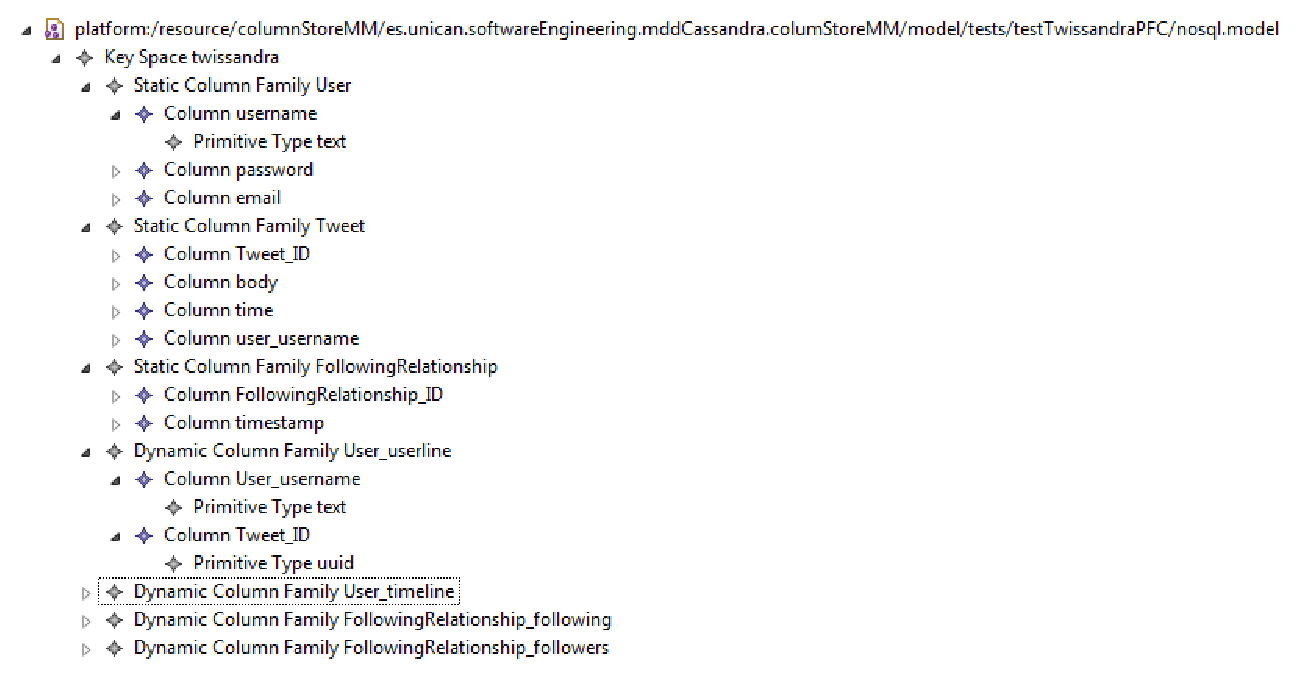
\includegraphics[width=.8\linewidth]{m2t/images/modeloTwissandra.eps} \\
  \caption{Modelo UML Twissandra}
  \label{back:fig:modeloTwissandra}
\end{figure}

Por cada column family (sea est�tica o din�mica) se genera un bloque "CREATE TABLE". Cada columna de la column family es un atributo de la tabla. El problema del generador de c�digo surge a la hora de definir la estructura de la primary key. Como se coment� en secciones anteriores las column family est�ticas siguen una definici�n de claves tradicional, sin embargo las column family din�micas tienen que tener en cuenta que las claves de partici�n (partition keys) pueden ser compuestas (aunque en este ejemplo no existen). Por ejemplo el caso de user\_userline las columnas user\_name y tweet\_id son designadas como primary key, user\_username ser� la clave de partici�n.
El c�digo resultante tras ejecutar el generador de c�digo es el siguiente figura~\ref{back:code:codigoCass}

\begin{figure}[!tb]
\begin{center}
\begin{footnotesize}
\begin{verbatim}
DROP KEYSPACE twissandra;
CREATE KEYSPACE twissandra
WITH replication = {'class':'SimpleStrategy', 'replication_factor':1};

USE twissandra;

CREATE TABLE User(
       username text,
       password text,
       email set<text>,
       PRIMARY KEY(username)
);

CREATE TABLE Tweet(
       Tweet_ID uuid,
       body text,
       time timestamp,
       user_username text,
       PRIMARY KEY(Tweet_ID)
);

CREATE TABLE FollowingRelationship(
       FollowingRelationship_ID uuid,
       timestamp timestamp,
       PRIMARY KEY(FollowingRelationship_ID)
);

CREATE TABLE User_userline(
       User_username text,
       Tweet_ID uuid,
       PRIMARY KEY((User_username),Tweet_ID)
);

CREATE TABLE User_timeline(
       User_username text,
       Tweet_ID uuid,
       PRIMARY KEY((User_username),Tweet_ID)
);

CREATE TABLE FollowingRelationship_following(
       FollowingRelationship_FollowingRelationship_ID uuid,
       username text,
       PRIMARY KEY((FollowingRelationship_FollowingRelationship_ID),username)
);

CREATE TABLE FollowingRelationship_followers(
       FollowingRelationship_FollowingRelationship_ID uuid,
       username text,
       PRIMARY KEY((FollowingRelationship_FollowingRelationship_ID),username)
);

\end{verbatim}
\end{footnotesize}
\end{center}
\caption{C�digo resultante}
\label{back:code:codigoCass}
\end{figure} 

\section{Pruebas}
\label{m2t:sec:pr}
%%==========================================================================%%
%% Author : Abascal Fern�ndez, Patricia                                     %%
%% Author : S�nchez Barreiro, Pablo                                         %%
%% Version: 1.1, 15/05/2013                                                 %%
%%                                                                          %%
%% Memoria del Proyecto Fin de Carrera                                      %%
%% Application Engineering/Pruebas                                          %%
%%==========================================================================%%

Una vez implementados los generadores de c�digo para la fase de \emph{Ingenier�a de Aplicaciones}, el siguiente paso era dise�ar y ejecutar las pruebas necesarias que permitiesen comprobar el correcto funcionamiento de estos generadores. Para dise�ar las pruebas,  siguiendo el mismo procedimiento que en el caso anterior, utilizando la t�cnica de clases de equivalencia y valores l�mites, para luego completar con casos espec�ficos que permitiesen alcanzar el 100\% de la cobertura.  

A diferencia de la fase de \emph{Ingenier�a del Dominio}, en esta fase no se utiliz� \emph{EUnit} para ejecutar dichas pruebas, ya que dicha herramienta no se ajustaba a nuestras necesidades. Por tanto, se crearon los casos de prueba y se ejecutaron a mano, analizando de forma tambi�n manual si la salida producida coincid�a con la esperada. La Tabla~\ref{app:table:pruebas} muestra algunos de los casos de prueba ejecutados.

\begin{table}
\begin{small}
\begin{tabularx}{\linewidth}{|X|l|}
 \hline
{Casos v�lidos}&{Casos no v�lidos} \\ \hline
Configuraci�n con un solo camino hoja-raiz & Paquetes recursivos. \\
Configuraci�n con varios caminos y todos los m�todos independientes &\\
Configuraci�n con varios caminos y alg�n m�todo dependiente &\\
Configuraci�n con varios caminos, donde alg�n m�todo tiene versiones dependientes e independientes &\\
\hline
\end{tabularx}
\end{small}
\caption{Casos de prueba para la fase de Ingenier�a de la Aplicaci�n}
\label{app:table:pruebas}
\end{table}%

Una vez creados y probados los generadores de c�digo, el siguiente paso era empaquetarlos para posibilitar su distribuci�n y uso. La siguiente secci�n describe como se realiza dicha fase de despliegue.
Tras ejecutar estos casos de prueba y comprobar que los generadores de c�digo funcionaban correctamente, d�bamos por concluida la labore de desarrollo de los generadores de c�digo, restando solo su empaquetado y despliegue.



\section{Despliegue}
\label{m2t:sec:des}
%%==================================================================%%
%% Author : Sa�udo Olmedo, Ignacio                                  %%
%% Author : S�nchez Barreiro, Pablo                                 %%
%% Version: 1.5, 15/05/2014                                         %%
%%                                                                  %%
%% Memoria del Proyecto Fin de Carrera                              %%
%% m2t/Sumario                                                      %%
%%==================================================================%%

Durante este cap�tulo se ha descrito el proceso de desarrollo del generador de c�digo. En primer lugar se ha presentado el c�digo del generador de c�digo y parte de la sintaxis utilizada para construirlo as� como la descripci�n de su realizaci�n. A continuaci�n se ha descrito el proceso de transformaci�n del caso de estudio introducido en el cap�tulo dos. Finalmente se han presentado las pruebas realizadas as� comola herramienta utilizada.   

\section{Sumario}
\label{m2t:sec:sumario}
%%==================================================================%%
%% Author : Abascal Fern�ndez, Patricia                             %%
%%          S�nchez Barreiro, Pablo                                 %%
%% Version: 1.1, 21/06/2013                                         %%
%%                                                                  %%
%% Memoria del Proyecto Fin de Carrera                              %%
%% Antecedentes, Sumario                                            %%
%%==================================================================%%

Durante este cap�tulo se han descrito los conceptos necesarios para comprender el �mbito y el alcance de este proyecto. Se ha descrito el caso de estudio que se utilizar� a lo largo del documento. A continuaci�n, se ha especificado qu� es una l�nea de productos software, el dise�o orientado a caracter�sticas, la metodolog�a TENTE, las limitaciones de las clases parciales en C\#, c�mo pueden resolverse estas limitaciones mediante el uso del \emph{SlicerPattern} y el proceso de generaci�n de c�digo con Epsilon.



